\documentclass{article}%
\usepackage[T1]{fontenc}%
\usepackage[utf8]{inputenc}%
\usepackage{lmodern}%
\usepackage{textcomp}%
\usepackage{lastpage}%
\usepackage[head=40pt,margin=0.5in,bottom=0.6in]{geometry}%
\usepackage{graphicx}%
%
\title{\textbf{Foro Penal registró 286 presos políticos actualmente en Venezuela}}%
\author{EL NACIONAL WEB}%
\date{20/11/2018}%
%
\begin{document}%
\normalsize%
\maketitle%
\textbf{URL: }%
http://www.el{-}nacional.com/noticias/presos{-}politicos/foro{-}penal{-}registro{-}286{-}presos{-}politicos{-}actualmente{-}venezuela\_260458\newline%
%
\textbf{Periodico: }%
EN, %
ID: %
260458, %
Seccion: %
Presos políticos\newline%
%
\textbf{Palabras Claves: }%
Política, Gobierno\newline%
%
\textbf{Derecho: }%
1.2%
, Otros Derechos: %
1.10, 5%
, Sub Derechos: %
1.2.2, 1.10.1%
\newline%
%
\textbf{EP: }%
NO\newline%
\newline%
%
\textbf{\textit{El organismo publicó la lista del balance de las cifras de arrestos, liberaciones, deportaciones y muertes en Venezuela}}%
\newline%
\newline%
%
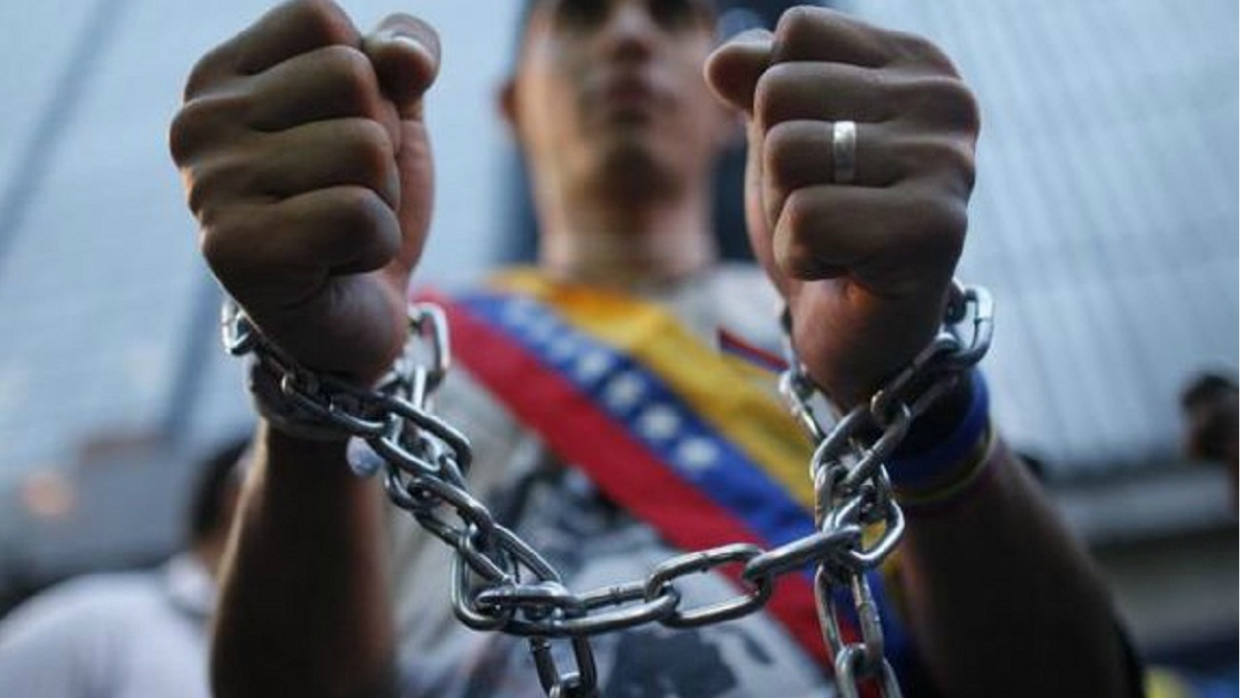
\includegraphics[width=300px]{195.jpg}%
\newline%
%
El Foro Penal Venezolano~denunció que desde el inicio de esta semana se han registrado 286 presos políticos en Venezuela de los cuales 61 tienen boleta de excarcelación.%
\newline%
%
En los datos del registro indican que de 286 presos, 80 son militares y 206 son personas civiles. "Desde el inicio de esta semana registramos en el Foro Penal 286 presos políticos en Venezuela. 61 tienen boleta de excarcelación", indicó Gonzalo Himiob, director de la ONG.%
\newline%
%
Destacan que 7505 personas se mantienen sujetas a procesos penales injustos por motivos políticos, bajo medidas cautelares.%
\newline%
%
\end{document}